%
% Last Revision: $Rev$
% Revision date: $Date$
% Author: $Author$
%
%\documentclass[10pt, openany]{report}
\documentclass[10pt, openany]{article}

\usepackage{fancyhdr}
\usepackage{multind}
\usepackage{geometry}
\usepackage{longtable}
\usepackage{color}
\usepackage[english]{isodate}
\geometry{letterpaper}
%
% Rules to allow import of graphics files in EPS and PDF format
%
\usepackage{pstricks}
\usepackage{graphicx}
\DeclareGraphicsExtensions{.eps}
\DeclareGraphicsRule{.eps}{eps}{.eps}{}
\DeclareGraphicsExtensions{.pdf}
\DeclareGraphicsRule{.pdf}{pdf}{.pdf}{}
\DeclareGraphicsExtensions{.png}
\DeclareGraphicsRule{.png}{png}{.png}{}
%
% Rules to add a "DRAFT" watermark to the output.
%
\usepackage{graphicx}
\usepackage{type1cm}
\usepackage{eso-pic}
\makeatletter
\newcommand{\watermark}[1]{
\AddToShipoutPicture{%
            \setlength{\@tempdimb}{.5\paperwidth}%
            \setlength{\@tempdimc}{.5\paperheight}%
            \setlength{\unitlength}{1pt}%
            \put(\strip@pt\@tempdimb,\strip@pt\@tempdimc){%
        \makebox(0,0){\rotatebox{45}{\textcolor[gray]{0.75}%
        {\fontsize{6cm}{6cm}\selectfont{#1}}}}%
            }%
}}
\makeatother
%\watermark{Draft}
%
% Other commands
%
\newcommand{\comment}[1]{\color{red}#1}
%
% Setup page headers and footers
%
\fancypagestyle{plain}
{
  \fancyhf{}
  \fancyhead[L]{Air Pressure Gradient in a Rotating Space Station}
  \chead{}
  \rhead{}
  \fancyfoot[L]{Personal Investigation}
  \fancyfoot[R]{Page \thepage}
  \renewcommand{\headrulewidth}{0.4pt}
  \renewcommand{\footrulewidth}{0.4pt}
}

\pagestyle{fancy}
\fancyhead{}
\lhead{Air Pressure Gradient in a Rotating Space Station}
\chead{}
\rhead{}
\lfoot{Personal Investigation}
\cfoot{Brent Seidel}
\rfoot{Page \thepage}
\renewcommand{\headrulewidth}{0.4pt}
\renewcommand{\footrulewidth}{0.4pt}
%
% Front Matter
%
\title{Air Pressure Gradient in a Rotating Space Station}
\author{Brent Seidel}
\date{ \today }
%========================================================
%%% BEGIN DOCUMENT
\begin{document}
\maketitle
\begin{abstract}
A formula for computing the air pressure at various distances from the center of a rotating space station is developed.
\end{abstract}
\tableofcontents
\listoffigures
\addcontentsline{toc}{section}{List of Figures}
\listoftables
\addcontentsline{toc}{section}{List of Tables}
%========================================================
\section{Introduction}

Artificial gravity in a radially symmetric space station can be created by rotating it around its axis.  From this, it is theoretically possible to construct a space station with roughly earth-like conditions on the inside surface.  This idea has been explored in fiction, most notably \emph{2001: A Space Odyssey}\cite{Kubrick:1968ve} and \emph{Babylon 5}\cite{:1993dq}.  The book \emph{Eon}\cite{Bear:1985fj}, describes a hollowed out asteroid rotating to produce artificial gravity.  In this case the air pressure is less than earth normal and the rotation produces about 0.6 of earth's gravity.  Larry Niven's \emph{Ringworld}\cite{Niven:1977rz} is perhaps the ultimate expression of a rotating cylinder space station with a radius equal to about one AU.

A formula giving the air pressure at any distance from the center of a rotating space station is desired.

%========================================================
\section{Development}
The coordinates in the space station are $x$, the distance along the axis, $r$, the distance from the axis of rotation, and $\theta$, the angle from a fixed reference point.  Note that this coordinate system is rotating.  A number of parameters and constants are defined in Table~\ref{tbl:Param}.

\begin{table}[ht]
\centering
\caption{Definition of Parameters}
\vspace{1ex}
\label{tbl:Param}
\begin{tabular}{|l|l|l|l|}
\hline
Parameter & Description & Value & Dimensions\\ \hline
$r$ & Distance from axis of rotation & & $m$\\ \hline
$R_{1}$ & Radius of space station & & $m$\\ \hline
$A_{0}$ & Acceleration at $R_{1}$ & 9.8 & $m \times s^{-2}$\\ \hline
$\Delta V$ & Small volume & $r \times \Delta x \times \Delta r \times \Delta\theta$ & $m^{3}$\\ \hline
$\omega_{0}$ & Angular velocity of space station & $\sqrt{\frac{A_{0}}{R_{1}}}$ & $radians^{2}$\\ \hline
$p$ & Air pressure & & $kPa$\\ \hline
$P_{1}$ & Air pressure at outside inner surface & 101.325 & $kPa$\\ \hline
$V$ & Volume & & $m^{3}$\\ \hline
$n$ & Number of molecules & & $mol$\\ \hline
$R$ & Ideal gas constant & 8.314472 & $J \times K^{-1} \times mol^{-1}$\\ \hline
$T$ & Temperature & 293.15 & $K$\\ \hline
$M$ & Molar mass of the gas & & $g \times mol^{-1}$\\ \hline
$M_{air}$ & Approximate molar mass of air & 0.029 & $kg \times mol^{-1}$\\ \hline
\end{tabular}
\end{table}

The centripetal force is given by:
\begin{equation}\label{eq:Force}
F=mr\omega^2
\end{equation}

With some manipulation of (\ref{eq:Force}), the angular velocity can be determined to be:
\begin{equation}\label{eq:Angular}
\omega_{0} = \sqrt{\frac{A_{0}}{R_{1}}}
\end{equation}

The ideal gas law is:
\begin{equation}\label{eq:Gas}
pV=nRT
\end{equation}

The mass of a quantity of gas is given by:
\begin{equation}\label{eq:Mass}
m = nM
\end{equation}

Assuming that air consists of 75\% Nitrogen and 25\% Oxygen, we have a molar mass of air ($M_{air}$) approximately 29 g/mol.

Substituting (\ref{eq:Mass}) into (\ref{eq:Gas}) and solving for mass gives:
\begin{equation}\label{eq:MassGas}
m=\frac{pVM_{air}}{RT}
\end{equation}

Substituting (\ref{eq:MassGas}) into (\ref{eq:Force}) gives the force (weight) of a small volume of gas:
\begin{equation}\label{eq:ForceGas}
F = \frac{p\Delta VM_{air}r\omega^2}{RT}
\end{equation}

Since pressure is force divided by area, we can obtain the pressure contribution of this small volume as:
\begin{equation}\label{eq:Press1}
\Delta p = \frac{\Delta F}{\Delta x \times r\Delta\theta} = \frac{pM_{air}\omega^{2}}{RT} \times \frac{r \times \Delta x \times \Delta r \times r\Delta\theta}{r \times \Delta x \times \Delta\theta}
\end{equation}

Simplifying and canceling (\ref{eq:Press1}) and substituting the angular velocity from \ref{eq:Angular} gives:
\begin{equation}\label{eq:Press2}
\Delta p =  \frac{pM_{air}A_{0}}{RTR_{1}} r\Delta r
\end{equation}

Since $M_{air}$, $A_{0}$, $R$, $T$, and $R_{1}$ are constants and $p$ is a function of $r$, (\ref{eq:Press2}) can be rewritten as:
\begin{equation}\label{eq:Press3}
\Delta p = k p(r) r\Delta r
\end{equation}

Where
\begin{equation}\label{eq:Constants}
k = \frac{M_{air}A_{0}}{R_{1}RT}
\end{equation}

Plugging in known values and canceling units in (\ref{eq:Constants}) gives:
\begin{equation}\label{eq:ConstNum}
k = \frac{0.029 \frac{kg}{mol} \times 9.8 \frac{m}{s^{2}}}{R_{1} \times 8.314472 \frac{J}{K \times mol} \times 293.15 K} = \frac{1.662 \times 10^{-4}}{R_{1}}\times m^{-1}
\end{equation}

Taking the limit of (\ref{eq:Press3}) as $\Delta r$ approaches zero give the differential equation:
\begin{equation}\label{eq:Press4}
dp = kp rdr
\end{equation}

This has a solution of the form:
\begin{equation}\label{eq:Solution}
p(r) = Ce^{\frac{kr^{2}}{2}}, p(R_{1}) = P_{1}
\end{equation}

The value of the constant $C$ can now be determined as:
\begin{equation}\label{eq:SolConst}
C=\frac{P_{1}}{e^{\frac{M_{air}A_{0}R_{1}}{2RT}}}
\end{equation}

Note that both constants, $k$ and $C$ are both functions of the size, $R_{1}$ of the space station, which gives a formula
\begin{equation}\label{eq:SolR1r}
p(R_{1}, r) = \frac{P_{1}}{e^{\frac{M_{air}A_{0}R_{1}}{2RT}}} \times e^{\frac{M_{air}A_{0}r^{2}}{2R_{1}RT}}
\end{equation}

This can be rewritten as:
\begin{equation}\label{eq:SolMod}
p(R_{1}, r) = P_{1}e^{\frac{M_{air}A_{0}(r^{2}-R_{1}^{2})}{2R_{1}RT}}
\end{equation}

Putting in numbers where possible gives (note that $R_{1}$ and $r$ are in meters):
\begin{equation}\label{eq:SolNum}
P(R_{1}, r) = 101.325kPa\times e^{\frac{5.83 \times 10^{-5}(r^{2}-R_{1}^{2})}{R_{1}}}
\end{equation}


A contour plot of this function is shown in Figure~\ref{fig:PressContour}.  The air pressures are given in kPa, where standard atmospheric pressure is slightly greater than 100 kPa.  Figure~\ref{fig:PressAxis} shows the air pressure at the axis of the station for various sizes of the station.  For comparison, elevations for some air pressures are given in Table~\ref{tbl:AirPress}.

\begin{figure}[!ht] 
  \centering
  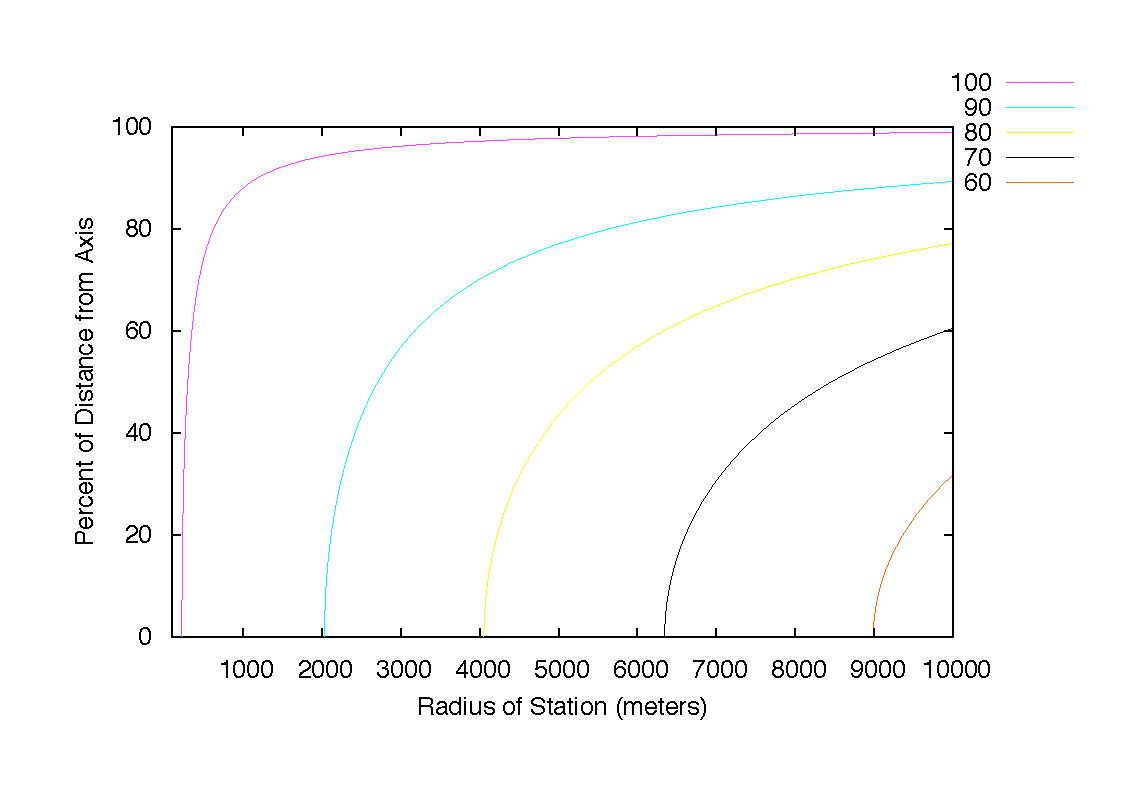
\includegraphics[scale=0.7]{fig1.pdf}
  \vspace{1ex}
  \caption{Air Pressure Curves for Various Space Station Sizes}
  \label{fig:PressContour}
\end{figure}

\begin{figure}[!ht] 
  \centering
  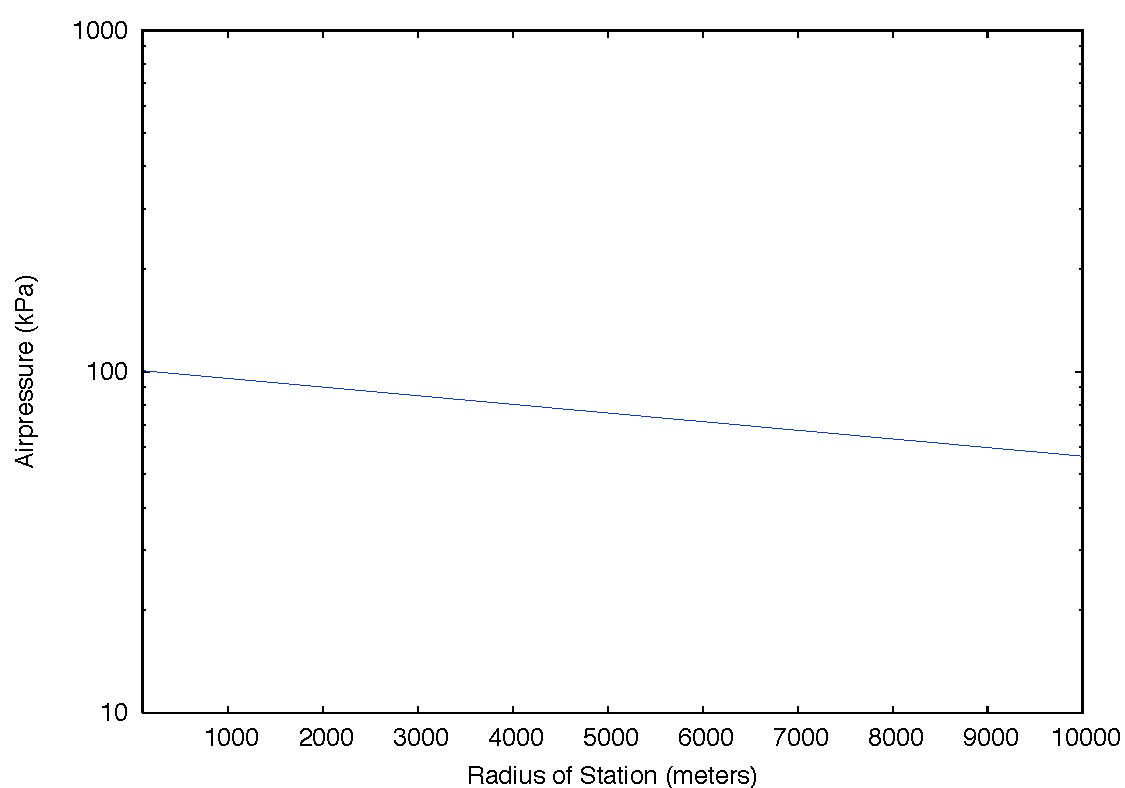
\includegraphics[scale=0.7]{fig2.pdf}
  \vspace{1ex}
  \caption{Air Pressure at Axis for Various Space Station Sizes}
  \label{fig:PressAxis}
\end{figure}

\begin{table}[ht]
\centering
\caption{Air Pressure per Elevation on Earth}
\vspace{1ex}
\label{tbl:AirPress}
\begin{tabular}{|l|l|}
\hline
Pressure (kPa) & Altitude (ft\\ \hline
100 & Sea Level\\ \hline
80 & 6600\\ \hline
60 & 14500\\ \hline
40 & 24750\\ \hline
20 & 41000\\ \hline
\end{tabular}
\end{table}

%========================================================
\section{Conclusions}
The air at the center of a rotating space station should be easily breathable for stations up to about 4000 meters in radius.  People would be able to acclimatize to the air pressure at the center of a 9000 meters radius station.

For a sufficiently large station, the decrease in pressure would reduce the need for pressure sealing along the axis.  Larry Niven's \emph{Ringworld}\cite{Niven:1977rz} is a rather extreme example of this situation.

Note that the pressures given should be considered an approximation.  There will no doubt be fluctuations due to weather and similar effects.  Also, temperature has been assumed to be constant.  Further investigation could be done to consider the effects of temperature varying with altitude.
%
% Setup bibliography
%
\clearpage
%========================================================
\addcontentsline{toc}{section}{References}
\bibliography{Bibleography}
\bibliographystyle{alpha}

\end{document}